\documentclass[10pt]{beamer}
% Use metropolis if installed, otherwise a clean default setup.
\IfFileExists{beamerthememetropolis.sty}{%
  \usetheme{metropolis}%
}{%
  \usetheme{default}%
  \usecolortheme{seagull}%
  \setbeamertemplate{navigation symbols}{}%
  \setbeamertemplate{footline}[frame number]%
  \setbeamerfont{frametitle}{series=\bfseries}%
}
\usepackage{booktabs}
\usepackage{array}

\newcommand{\code}[1]{\texttt{#1}}

\title{TAPLite Kernel Computational-Efficiency Enhancements}
\subtitle{Warm Starts, SP-Tree Sharing, and Column Stores}
\author{Xuesong Zhou \and TAPLite4MPO team}
\date{July 2026}

\begin{document}

\begin{frame}
  \titlepage
\end{frame}

\begin{frame}{Headline: what this buys the looped 4-step process}
  \footnotesize
  Assignment runs \textbf{once per global feedback loop}
  (typically 4--8 loops $\times$ 5 periods = 20--40 calls); all entries from
  our measured numbers, derived rows labeled.
  \begin{center}
  \scriptsize
  \begin{tabular}{p{0.28\textwidth}p{0.27\textwidth}p{0.33\textwidth}}
    \toprule
    Lever & Factor & Basis \\
    \midrule
    1. L1 within-loop warm start (shipped) & \textbf{$\sim$45\% fewer iters}
      ($\sim$11 vs 20); \textbf{1.9x tighter} &
      Measured: SCAG AM L1 table \\
    2. L2 loop-over-loop restart (shipped) & \textbf{2.2x} per call
      (35\,s vs 78\,s); starts \emph{at} prior gap 0.072\% &
      Measured: SCAG AM L2 table \\
    3. Whole feedback run & \textbf{$\sim$1.8x} warm starts alone &
      Derived: rows 1--2 \\
    4. L3 column replay + GP sweeps (shipped) & \textbf{139x} to 0.10\% gap;
      \textbf{8.4x} to 0.05\%; $\leq$0.02\% \emph{only} via GP &
      Measured: SCAG same-gap table (compute-only) \\
    \bottomrule
  \end{tabular}
  \end{center}
  \scriptsize
  Derived arithmetic: 5-loop run $= 5T$ cold vs
  $T + 4 \times 0.45T \approx 2.8T$ $\Rightarrow$ $\sim$1.8x for the full
  feedback run. Multi-class runs save another
  2--3x on SP via tree sharing (6 modes $\rightarrow$ 4 trees, byte-identical);
  all numbers sit on the 30/30 regression + byte-identity gate.

  \smallskip
  \emph{The kernel's shortest-path engine was modernized to industry-standard
  heap label-setting (21x on our prior internal baseline) --- treated here as
  a prerequisite, not a claimed advance.}
\end{frame}

\begin{frame}{Motivation}
  \begin{itemize}
    \item Regional assignment runs are rarely one-off: VDF recalibration,
      toll tweaks, demand scenarios, gap-tightening continuations.
    \item A cold Frank--Wolfe start rediscovers congestion every time:
      \textbf{SCAG RTP24 AM iteration-1 gap = 185\%} from free-flow times.
    \item Goal: reuse what the previous run already computed ---
      \emph{without} ever compromising exactness or trust.
    \item Method: a structured \textbf{industry panel} of five expert personas,
      each reviewing the actual kernel source.
  \end{itemize}
\end{frame}

\begin{frame}{The industry-panel method}
  Five personas, five traditions, one kernel (\code{TAPLite.cpp}):
  \begin{enumerate}
    \item Caliper-class commercial vendor engineer
    \item PTV/Visum-class commercial vendor engineer
    \item Open-source lead (AequilibraE-class)
    \item Bar-Gera-tradition academic (convergence theory)
    \item HPC/systems engineer (memory layout, binary formats)
  \end{enumerate}
  \medskip
  Each proposed accelerations with effort estimates and registered
  \emph{dissents}. The panel converged on one organizing artifact:
  the \textbf{warm-start ladder}.
\end{frame}

\begin{frame}{The warm-start ladder L1--L4}
  \begin{description}
    \item[L1 -- TIMES] Preload congested link times from a prior run.
      Feasibility untouched; equilibrium unchanged. All 5 endorse; ship first.
    \item[L2 -- FLOWS] Restore link volumes, skip iteration-0 AoN.
      Valid only for \emph{identical demand} (fingerprint-enforced).
    \item[L3 -- COLUMNS] Per-OD path sets with $\theta$ shares:
      a \emph{demand-invariant routing policy}, replayable against any new
      OD table. Unanimously ``the strategic asset.''
    \item[L4 -- STATE] mmap-able full snapshot (DTST); kills the input-parse
      phase. Planned.
  \end{description}
  \medskip
  Universal rule: reset CFW/BFW direction history on any warm start.
  Startup resolution: DTAC $\to$ L3, else DTLR $\to$ L2, else DTLP $\to$ L1,
  else free-flow --- every decision logged.
\end{frame}

\begin{frame}{P0 (shipped): the exact trio}
  All three verified \textbf{bit-identical} via byte-diffs of
  \code{link\_performance.csv} + gap trajectories vs the pre-change exe.
  \begin{itemize}
    \item \textbf{L1 \code{warm\_start\_times}}: preload congested times from a
      prior \code{link\_performance} CSV or DTLP binary, matched by external
      link id. Bad input $\Rightarrow$ loud warning, cold start; never fails.
    \item \textbf{SP-equivalence auto-detect}: modes share one tree iff
      \code{allowed\_use} and per-link additional cost are identical everywhere.
      PCE/occupancy never split a group. 6 modes $\to$ 4 trees on Chicago
      Sketch multimodal, byte-identical; grouping always logged.
    \item \textbf{Group-aware zero-demand-origin skip}: per-(mode, origin) SP
      skip with direct BIGM fill --- identical results by construction.
  \end{itemize}
  \medskip
  Regression: \textbf{30/30 checks pass, no re-baselining.}
\end{frame}

\begin{frame}{P0 evidence: SCAG RTP24 AM, 224{,}288 links}
  \begin{table}
  \centering
  \begin{tabular}{lrr}
    \toprule
     & Cold & L1 warm start \\
    \midrule
    Iteration-1 gap          & 185.2\%   & 44.9\% \\
    Iters to cold's final gap & 19       & $\sim$11 \\
    Final gap (iter 19)      & 0.0755\%  & \textbf{0.0407\%} \\
    \bottomrule
  \end{tabular}
  \end{table}
  \begin{itemize}
    \item $\sim$\textbf{1.9x tighter} final gap, $\sim$2x fewer iterations to
      equal gap.
    \item 224{,}288 / 246{,}806 links matched (connectors keep free-flow time
      by design).
    \item Only the starting point changes --- same equilibrium.
  \end{itemize}
\end{frame}

\begin{frame}{P1 (shipped): DTLR snapshot + \code{warm\_start\_flows}}
  \begin{itemize}
    \item \code{flow\_snapshot=1} writes \code{link\_flows.bin}
      (magic \code{DTLR}): main + per-mode volumes by external link id.
    \item Header carries a \textbf{16-byte demand fingerprint}: OD total,
      positive-cell count, min/max zone id --- deterministic accumulation.
    \item On match: restore volumes, recompute times, \emph{skip iteration-0
      AoN}, continue FW from iteration 1. The restored point is a convex
      combination of AoN assignments of the same demand $\Rightarrow$ a valid
      FW iterate.
    \item On mismatch (or wrong magic / mode count): \textbf{loud warning, both
      fingerprints printed, demote to L1} (times-only seed) --- never a silent
      restart from incompatible flows.
    \item Guard verified: one OD cell perturbed 10\% on Chicago Sketch flips
      the fingerprint and triggers the demotion.
  \end{itemize}
\end{frame}

\begin{frame}{P1 evidence: SCAG restart continuation}
  \begin{table}
  \centering
  \begin{tabular}{lrr}
    \toprule
     & Run A: cold, 20 it & Run B: warm, 10 it \\
    \midrule
    Links restored    & ---       & 246{,}806 / 246{,}806 \\
    Iteration-1 gap   & 185.23\%  & \textbf{0.0724\%} \\
    Final gap         & 0.0755\%  & \textbf{0.0453\%} \\
    FW wall time      & 78\,s     & \textbf{35\,s} \\
    \bottomrule
  \end{tabular}
  \end{table}
  \begin{itemize}
    \item Run B starts \emph{at} run A's final gap --- a seamless continuation.
    \item \textbf{1.7x tighter} gap in \textbf{0.45x} the wall time.
    \item Identical-demand reruns (recalibration, gap tightening) lose no work.
  \end{itemize}
\end{frame}

\begin{frame}{P2 increment 1 (shipped): DTAC column store}
  \code{column\_output=1} writes \code{route\_columns.bin} (magic \code{DTAC}),
  sparse CSR over positive-demand OD pairs: the \emph{last-iteration shortest
  path} per (mode, origin, destination) as external-link-id sequences.
  \begin{table}
  \centering
  \begin{tabular}{lr}
    \toprule
    Chicago Sketch (20 it, 3 modes, 387 zones) & \\
    \midrule
    Stored paths / link entries & 93{,}135 / 1{,}211{,}261 \\
    DTAC vs \code{route\_assignment.csv} & 5.6\,MB vs 55.1\,MB
      (\textbf{9.8x smaller}) \\
    Push-down $R^2$ vs link volumes & 0.9657 \\
    Turn-restriction single-path net & $R^2 = 1.0$, banned movement avoided \\
    \bottomrule
  \end{tabular}
  \end{table}
  \textbf{Honest caveat}: $R^2$ 0.966 is expected --- link volumes are the FW
  blend of 20 iterations; increment 1 stores only the final AoN direction.
  Exactness arrives with increment 2's $\theta$ shares.
\end{frame}

\begin{frame}{P2 increment 2 / full L3 (shipped): $\theta$ shares, replay, GP}
  \begin{itemize}
    \item \textbf{DTAC v2 $\theta$-share columns}: the path SET across all FW
      iterations, exact FW cascade $\Rightarrow$ push-down
      $R^2 = 1.000000$, max diff 0.00\,veh (increment 1: 0.9657).
    \item \textbf{\code{warm\_start\_columns}}: scatter $\theta \times$ the
      \emph{current} OD table --- demand \emph{may} differ (that is the point);
      paths broken by network edits dropped + $\theta$ renormalized;
      skip iteration-0 AoN, resume FW.
    \item \textbf{\code{column\_adjust\_sweeps}}: fixed-policy GP sweeps
      (Gauss--Seidel, exact VDF derivatives, no SP calls).
    \item \textbf{Mandatory two-gap report}: \emph{restricted} gap (stored
      paths) and \emph{TRUE} gap (fresh SP) always printed --- restricted
      never masquerades as UE. Freeze/replay = 0 FW iterations + same report.
  \end{itemize}
  \medskip
  Regression 30/30; defaults-off \code{link\_performance.csv} AND
  \code{route\_assignment.csv} byte-identical to the pre-change exe.
\end{frame}

\begin{frame}{L3 evidence: same-gap trade-off, SCAG RTP24 AM}
  \footnotesize
  246{,}806 links, 342{,}712 OD cells; demand perturbed $+5\%$ on 1{,}000
  cells. \textbf{Compute seconds} to a TRUE-gap target (setup + DTAC load
  excluded --- the accounting rule; kernel prints phase timings).
  \begin{center}
  \scriptsize
  \begin{tabular}{lrrrl}
    \toprule
    Target & Cold FW & Warm replay+FW & Warm + GP & Speedup \\
    \midrule
    0.10\% & 101.7\,s @ 15 it & 8.6\,s @ 1 it & 0.7\,s @ scatter & \textbf{139x} \\
    0.05\% & 183.4\,s @ 26 it & 28.5\,s @ 6 it & 21.9\,s @ 1 sweep & \textbf{8.4x} \\
    0.02\% & not reached (0.036\%) & not reached (0.033\%) & 21.9\,s @ 1 sweep & only GP \\
    0.01\% & not reached & not reached & 21.9\,s @ 1 sweep & only GP \\
    \bottomrule
  \end{tabular}
  \end{center}
  \medskip
  \textbf{The regime split}: plain FW --- cold OR warm-started --- plateaus
  above $\sim$0.03\%; GP sweeps over the stored columns pass 0.01\% in 1--3
  sweeps and keep going (8 sweeps $\to 7.6\times10^{-4}$\,\%). The sweeps
  reach targets FW cannot. Chicago Sketch: 4.8x @ 0.10\%, 2.4x @ 0.05\%,
  GP-only below.
\end{frame}

\begin{frame}{L3 evidence: the trade-off figure}
  \begin{center}
    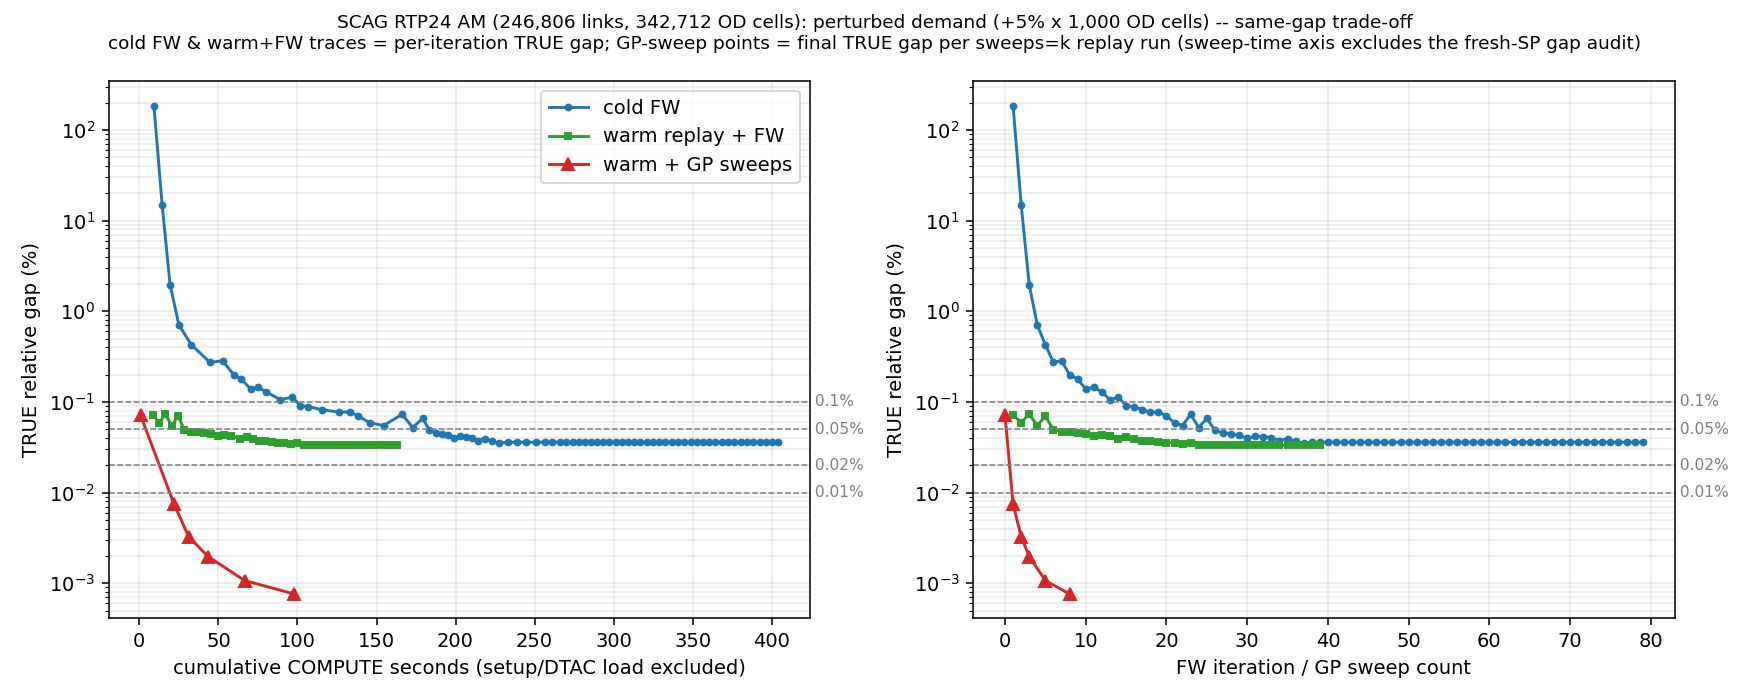
\includegraphics[width=\textwidth]{l3_tradeoff_scag.png}
  \end{center}
  \scriptsize
  FW curves = per-iteration TRUE gap; GP points = final TRUE gap of each
  sweeps$=k$ replay run. Companion: \code{l3\_tradeoff\_sketch.png}
  (Chicago Sketch, same regimes).
\end{frame}

\begin{frame}{The standard rerun recipe (team decision)}
  \begin{block}{Rerunning ANY model = L3 warm start to a 0.1\% gap}
    \code{warm\_start\_columns = route\_columns.bin}\\
    \code{convergence\_gap\_pct = 0.1}\\
    \code{column\_adjust\_sweeps = 0}
  \end{block}
  \begin{itemize}
    \item Baseline run sets \code{column\_output=1} once.
    \item Replay+FW reaches the 0.1\% TRUE gap in $\sim$1 iteration ---
      \textbf{139x} less compute than cold on SCAG.
    \item Add sweeps only for tighter targets (1 sweep $\to$ 0.01\% on SCAG).
    \item Kernel cold-start defaults unchanged; settings-only, opt-in.
    \item Full recipe + guard behavior:
      \code{github\_taplite/docs/RERUN\_RECIPE.md}.
  \end{itemize}
\end{frame}

\begin{frame}{The binary format family}
  \begin{table}
  \centering
  \small
  \begin{tabular}{llll}
    \toprule
    Magic & Role & Written by & Consumed by \\
    \midrule
    DTAB & OD demand & \code{demand-bin} tool & \code{demand\_format=1}
      (2.5--3x load) \\
    DTLP & Link performance & \code{link\_output=3} & L1 warm start; reporting \\
    DTLR & Flow restart & \code{flow\_snapshot=1} & L2
      \code{warm\_start\_flows} \\
    DTAC & Path columns (v2: $\theta$) & \code{column\_output=1} & verifier;
      L3 \code{warm\_start\_columns} \\
    DTST & Full state & \emph{planned} (L4) & \emph{planned}: mmap, skips
      input parse \\
    \bottomrule
  \end{tabular}
  \end{table}
  \medskip
  Common contract: magic + version headers, external-link-id matching,
  loud fallback on invalid input --- a run is never aborted by an
  optimization hint.
\end{frame}

\begin{frame}{Engineering principles}
  \begin{itemize}
    \item \textbf{Exact or clearly reported} --- bit-exact features, or a
      printed, quantified deviation (DTAC $R^2$; restricted-vs-full gap).
    \item \textbf{Default-off} --- every behavior-changing key ships off and is
      registered in the \code{dtalite\_qa} schema.
    \item \textbf{Loud-warn, never fail} --- bad warm-start input degrades
      gracefully (cold start or L1 demotion), with match rates logged.
    \item \textbf{Fingerprint guards} --- one perturbed OD cell flips the
      demand fingerprint and demotes the restart.
    \item \textbf{Regression + byte-identity gates} --- 13 networks / 30
      checks, no re-baselining, byte-diffs vs the pre-change exe.
    \item \textbf{No bush-based rewrite} --- unanimously rejected; GP polish on
      stored columns gives ``bush-method-class precision without becoming
      Algorithm B.''
  \end{itemize}
\end{frame}

\begin{frame}{Summary}
  \begin{itemize}
    \item \textbf{P0 shipped}: L1 times warm start + SP-tree sharing +
      origin skip --- all exact, 30/30 regression.
    \item \textbf{P1 shipped}: DTLR flow restart with demand-fingerprint
      guard --- SCAG restarts \emph{at} the prior final gap; 1.7x tighter in
      0.45x time.
    \item \textbf{P2/L3 shipped}: DTAC v2 $\theta$-share columns (push-down
      $R^2 = 1.000000$), rescale-to-new-OD replay, GP sweeps, freeze/replay
      with the mandatory two-gap report.
    \item \textbf{Same-gap headline (SCAG)}: 139x @ 0.10\%, 8.4x @ 0.05\%;
      $\leq$0.02\% only via GP (FW plateaus $\sim$0.03\%; GP $\to$
      $8\times10^{-4}$\,\%).
    \item \textbf{Standard rerun recipe}: \code{warm\_start\_columns} +
      0.1\% gap target + 0 sweeps --- every rerun, any demand.
    \item \textbf{Remaining}: per-origin parallel GP sweeps; L4 DTST state
      snapshot (kill the setup phase).
    \item The ladder compounds: every rung reuses the formats and guards of
      the one below it.
  \end{itemize}
\end{frame}

\end{document}
